\section{Results}
\label{sec:results}

\subsection{Reconstruction Quality}
\label{sec:results_reconstruction}

Table~\ref{tab:reconstruction_accuracy} reports decoder reconstruction accuracy on normal (non-attacked) test data, averaged across 5 cross-validation folds.

\begin{table}[t]
\centering
\caption{Reconstruction accuracy on normal test data. V8 entries are mean $\pm$ std across 5 folds, evaluated reference-conditioned (each step conditioned on the preceding ground-truth tokens), the same conditioning as the NLL detection scores. V7 entries are point estimates of mixed evaluation regime (note $^{a}$); the load-bearing comparison is the numeric accuracy, where V7 (free-running) resolves fewer than one numeric token in six. V8 trades lower overall token accuracy for substantially higher numeric (+26.7~pp) and command (+14.9~pp) accuracy, reflecting the harder multi-line task.}
\label{tab:reconstruction_accuracy}
\begin{tabular}{@{}lccc@{}}
\toprule
Metric & V7 & V8 & $\Delta$ (V8 $-$ V7) \\
\midrule
Token accuracy (overall) & 81.8\% & 67.2 $\pm$ 1.1\% & $-14.6$ pp \\
Numeric accuracy          & 16.7\% & 43.4 $\pm$ 1.2\% & $+26.7$ pp \\
Command accuracy          & 73.8\% & 88.7 $\pm$ 3.0\% & $+14.9$ pp \\
\bottomrule
\multicolumn{4}{@{}p{0.92\columnwidth}}{\footnotesize $^{a}$V7 numeric accuracy (16.7\%) is the free-running per-token value from the error taxonomy (Appendix~\ref{app:errors}, Experiment~9, 5-fold; $1-0.833$). The 81.8\% token figure is teacher-forced overall-token accuracy on a representative fold and is reported only to contrast V7/V8 task difficulty; command accuracy is of the same order ($\approx$74\% free-running).}
\end{tabular}
\end{table}

V7 achieves higher overall token accuracy (81.8\% vs.\ 67.2\%) because its shorter sequences (3 content tokens) present a simpler task.
This overall figure overstates reconstruction quality, however.
V7's numeric accuracy is only 16.7\%, meaning it correctly predicts fewer than one in six numeric tokens.
V7's overall accuracy derives primarily from special tokens (BOS, EOS, PAD) and parameter-type tokens rather than from the most informative numeric values.

V8 reverses this pattern, achieving 43.4\% numeric accuracy (2.6$\times$ V7) and 88.7\% command accuracy (+14.9~pp).
We attribute these gains to multi-line context, which lets the decoder infer subsequent coordinates from the sequential pattern (e.g., G1 X-10.0 Y5.0 followed by G1 X-10.5 Y5.0) rather than from sensor signals alone.

\subsection{Anomaly Detection Performance}
\label{sec:results_anomaly}

Table~\ref{tab:main_results} presents AUROC for each attack type, scoring method, and decoder.
All values are means across 5 folds.

\begin{table}[t]
\centering
\caption{AUROC by attack type, decoder, and scoring method (mean across 5 folds). Best per attack is \textbf{bolded}. V8 rank scores are omitted as the V8 decoder's longer sequences make rank scoring redundant with $S_{\max}$ (both capture within-axis ordering). V7 excels on structural attacks; V8 on semantic attacks; rank scoring on small coordinate perturbations.}
\label{tab:main_results}
\small
\setlength{\tabcolsep}{4pt}
\begin{tabular}{@{}lcccccc@{}}
\toprule
 & \multicolumn{3}{c}{V7 Decoder} & \multicolumn{2}{c}{V8 Decoder} & \\
\cmidrule(lr){2-4} \cmidrule(lr){5-6}
Attack & $S_{\text{mean}}$ & $S_{\max}$ & $S_{\text{rank}}$ & $S_{\text{mean}}$ & $S_{\max}$ & Best \\
\midrule
A1 cmd swap       & \textbf{.803}(.050) & .701(.075) & .500       & .581(.019) & .691(.084) & V7 mean \\[2pt]
A2 $\delta{=}.001$ & .697(.151) & .742(.124) & \textbf{.859}(.130) & .604(.012) & .743(.058) & V7 rank \\
A2 $\delta{=}.01$  & .694(.052) & .826(.049) & \textbf{.901}(.057) & .598(.007) & .764(.037) & V7 rank \\
A2 $\delta{=}.1$   & .676(.018) & .790(.024) & \textbf{.847}(.068) & .619(.008) & .785(.040) & V7 rank \\
A2 $\delta{=}1.0$  & .637(.028) & .707(.022) & .754(.051) & .639(.008) & \textbf{.861}(.032) & V8 max \\
A2 $\delta{=}50$   & .559(.037) & .610(.057) & .599(.078) & .621(.008) & \textbf{.797}(.035) & V8 max \\[2pt]
A3 param sub       & \textbf{.621}(.039) & .557(.044) & .500       & .541(.005) & .574(.017) & V7 mean \\[2pt]
A4 cross-op        & .366(.039) & .500       & .623(.027) & \textbf{.949}(.007) & .759(.035) & V8 mean \\
\bottomrule
\multicolumn{7}{@{}l}{\footnotesize AUROC mean~(std) across 5 folds. Best per row in \textbf{bold}. Leading zeros omitted.}
\end{tabular}
\end{table}

\paragraph{No single method dominates.}
The best scoring method varies by attack type: V7 $S_{\text{mean}}$ for structural attacks (A1, A3), V7 $S_{\text{rank}}$ for small coordinate perturbations (A2, $\delta \leq 0.1$~in), V8 $S_{\max}$ for large perturbations (A2, $\delta \geq 1.0$~in), and V8 $S_{\text{mean}}$ for cross-operation attacks (A4).
The results argue against relying on any single anomaly score.

\paragraph{V7 excels at structural attacks.}
V7 achieves AUROC = $0.803 \pm 0.050$ on A1 and 0.621 on A3, outperforming all V8 variants.
With only 3 content tokens, each token carries a large fraction of total NLL; a command swap (e.g., G1 $\to$ G0) produces an undiluted spike.
In V8, the same swap affects one token among 63, and $S_{\text{mean}}$ averages the spike away.

\paragraph{V8 excels at semantic attacks.}
V8 achieves AUROC = 0.949 on A4 with $S_{\text{mean}}$, versus V7's 0.366.
The V7 result falls below chance, indicating an inverse correlation.
V7 assigns \emph{lower} NLL to cross-operation G-code than to the original, likely because foreign sequences are simpler and easier to predict regardless of sensor context.
V8 avoids this failure through multi-line context, under which cross-operation blocks receive high NLL.

\paragraph{Rank-based scoring outperforms NLL for coordinate attacks.}
On A2 with $\delta = 0.001$~in, V7 Rank achieves AUROC = 0.859 versus V7 NLL = 0.697 (+16.2~pp; pooled DeLong test $p = 1.2\times10^{-5}$, Holm--Bonferroni-corrected).
This advantage holds and strengthens across magnitudes up to $\delta = 0.1$~in (+20.7~pp at $\delta = 0.01$, Holm-adjusted $p = 5.1\times10^{-15}$; +17.1~pp at $\delta = 0.1$, Holm-adjusted $p = 1.1\times10^{-13}$). Rank-based scoring detects relative probability reordering regardless of absolute scale (Section~\ref{sec:rank_score}).

Rank scoring operates only on numeric tokens within a single axis. Command swaps (A1) and parameter substitutions (A3) modify non-numeric tokens, which rank scoring ignores by design. The 0.500 AUROC on A1 and A3 reflects this architectural choice, not a model failure.

Figure~\ref{fig:roc_curves} shows ROC curves for four representative attacks.
Figure~\ref{fig:score_distributions} shows score distributions for normal versus attacked windows.

\begin{figure}[t]
\centering
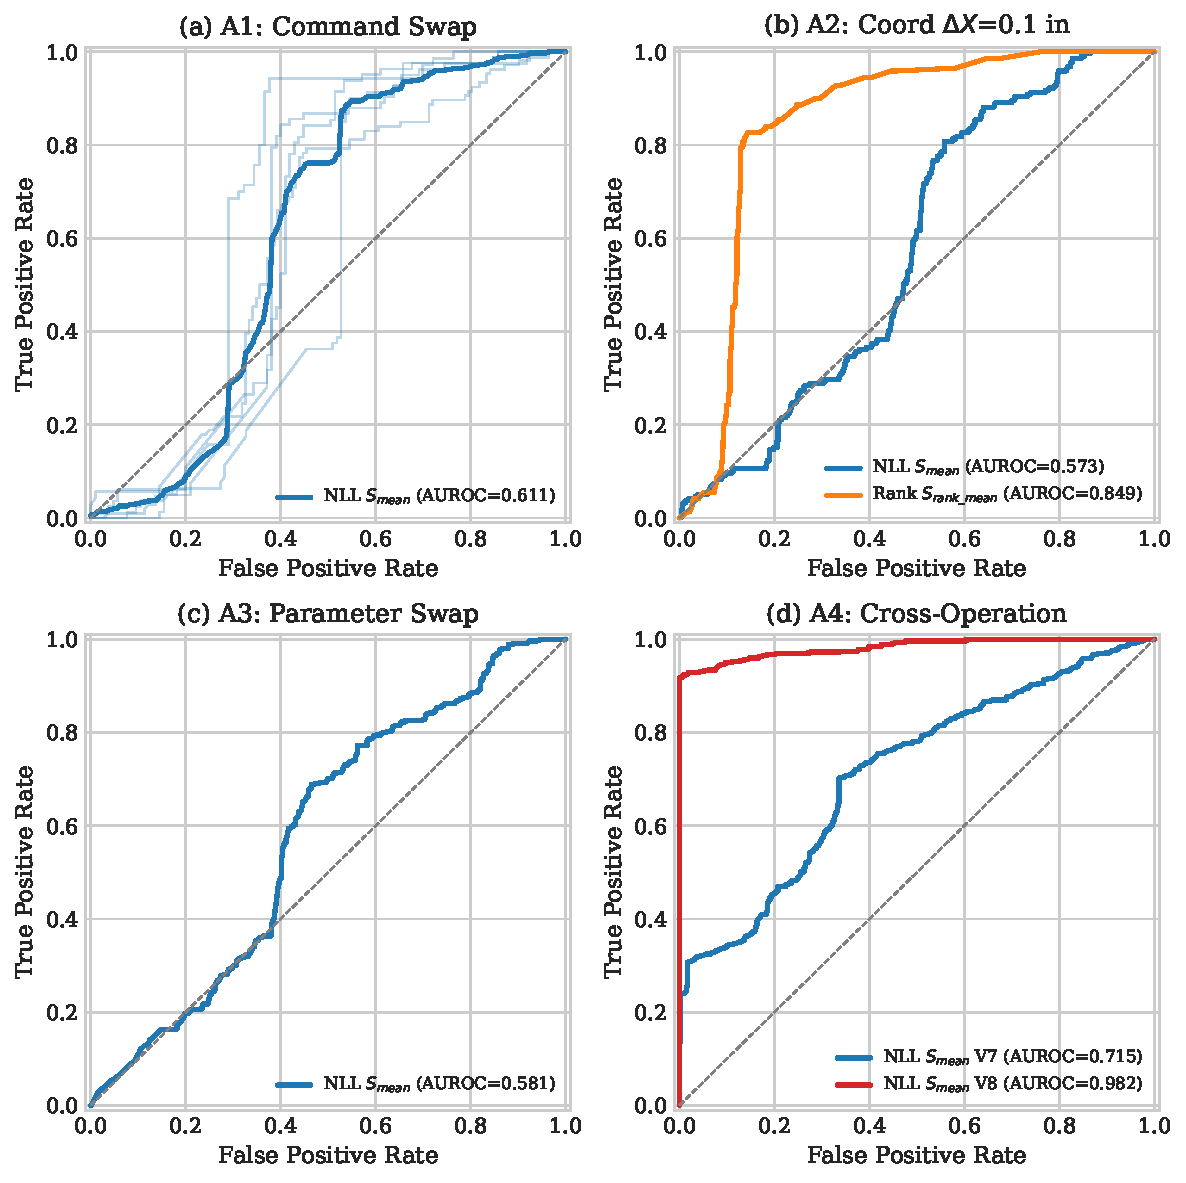
\includegraphics[width=\columnwidth]{figures/roc_curves.pdf}
\caption{ROC curves for four attack types. (a)~A1 command swap: per-fold curves (thin) and mean (thick). (b)~A2 coordinate perturbation ($\delta = 0.1$~in): NLL (blue) vs.\ rank scoring (orange), showing rank's clear advantage. (c)~A3 parameter swap. (d)~A4 cross-operation swap: V7 (blue) vs.\ V8 (red), showing V8's improvement from multi-line context.}
\label{fig:roc_curves}
\end{figure}

\begin{figure}[t]
\centering
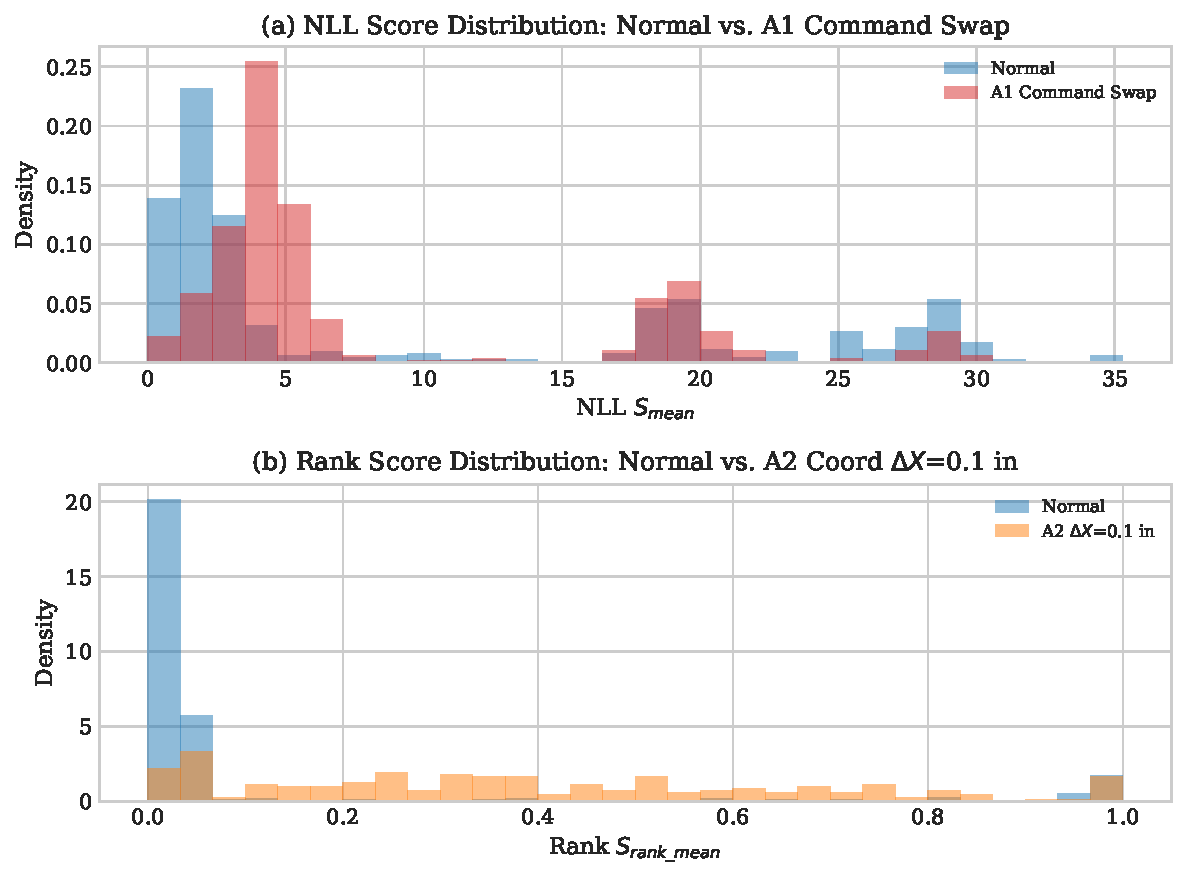
\includegraphics[width=\columnwidth]{figures/score_distributions.pdf}
\caption{Score distributions for normal (blue) vs.\ attacked (red/orange) windows. (a)~NLL $S_{\text{mean}}$: the spread of the normal distribution reflects the per-token confidence gradient (Section~\ref{sec:results_two_populations}). (b)~Rank $S_{\text{rank}}$: clear separation between normal and coordinate-attack windows.}
\label{fig:score_distributions}
\end{figure}

\paragraph{Perturbation-magnitude dependence.}
Larger perturbations are not always easier to detect.
Under V7, $S_{\text{rank}}$ AUROC drops from 0.859 ($\delta = 0.001$) to 0.599 ($\delta = 50$~in) because large perturbations push the axis value into a regime where the decoder's distribution is nearly uniform.
In that regime, both the original and perturbed values become equally implausible.
V8 partially recovers at large $\delta$ ($S_{\max}$ AUROC = 0.797) because multi-line context constrains the plausible coordinate range, so a coordinate far outside the range implied by surrounding lines produces a large $S_{\max}$ value.
Figure~\ref{fig:detection_vs_delta} traces this relationship across five perturbation magnitudes and four scoring methods.

\begin{figure}[t]
\centering
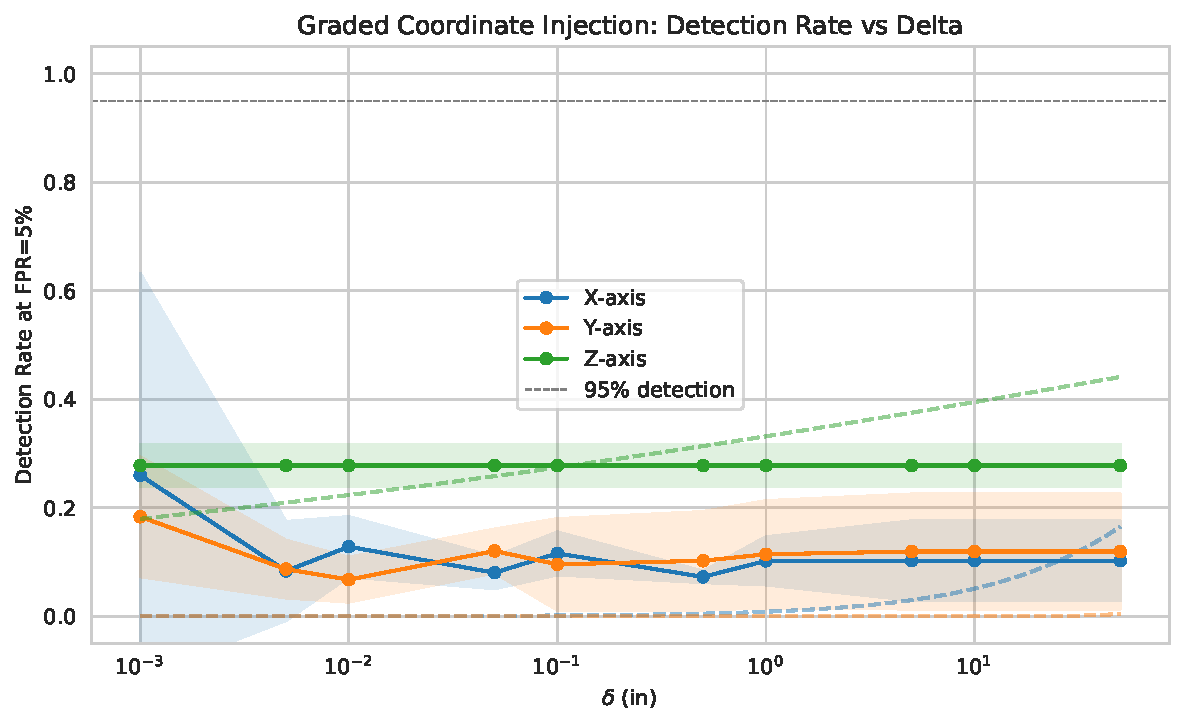
\includegraphics[width=\columnwidth]{figures/detection_vs_delta.pdf}
\caption{Detection AUROC vs.\ perturbation magnitude for X-axis coordinate attacks (A2). V7 rank scoring (orange) dominates at small $\delta$; V8 $S_{\max}$ (red dashed) recovers at large $\delta$ where rank scoring fails. Shaded bands show $\pm$1 std across 5 folds.}
\label{fig:detection_vs_delta}
\end{figure}

\begin{figure}[t]
\centering
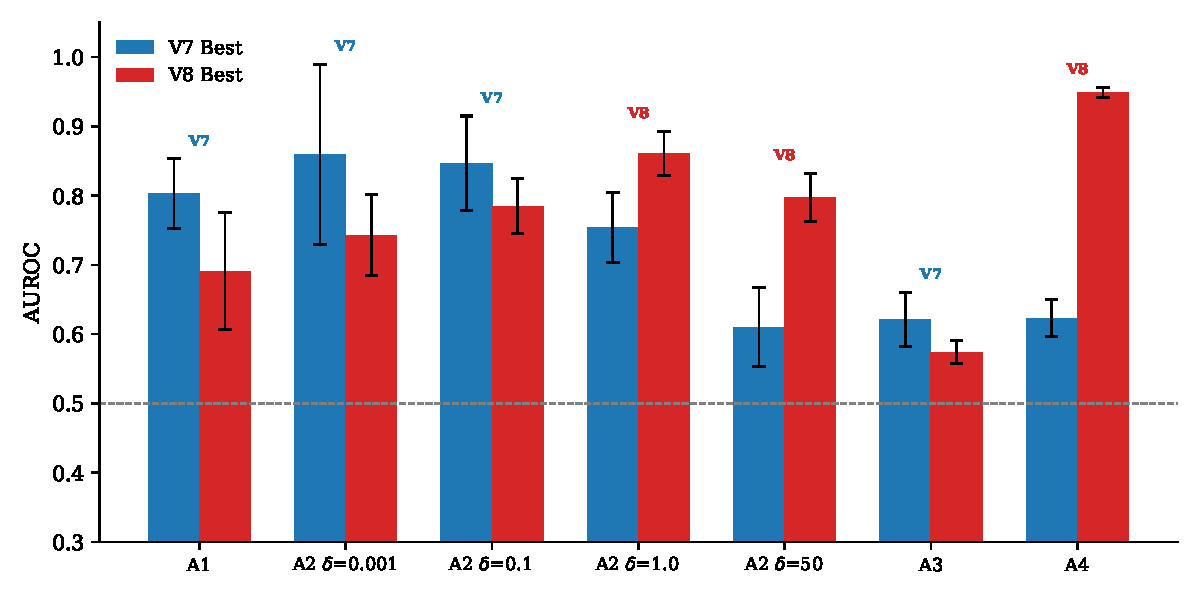
\includegraphics[width=\columnwidth]{figures/v7_v8_comparison.pdf}
\caption{Best AUROC per attack type for V7 (blue) vs.\ V8 (red) decoders. V7 dominates on structural attacks (A1, A3) and small coordinate perturbations; V8 dominates on large perturbations and cross-operation swaps.}
\label{fig:v7_v8_comparison}
\end{figure}

\paragraph{Axis dependence.}
X-axis perturbations are most detectable (V7 AUROC = 0.697 at $\delta = 0.001$), followed by Y (0.640) and Z (0.542).
Z-axis $S_{\text{mean}}$ AUROC is \emph{bit-identical} (0.542) across all ten magnitudes from 0.001 to 50~in.
This exact invariance is a tokenization artifact rather than a detectability plateau.
Z values are sparse in the corpus (depth changes are infrequent), so most Z perturbations round back to the original token and produce no change.
We therefore restrict coordinate-attack claims to the X and Y axes, where the vocabulary is dense enough to realize the requested perturbation.

\subsection{Encoder vs.\ Decoder Detection}
\label{sec:results_enc_dec}

Table~\ref{tab:encoder_vs_decoder} compares encoder-only and decoder-based detection.

\begin{table}[t]
\centering
\caption{Encoder-only vs.\ decoder-based detection on A1 command-swap attacks (mean $\pm$ std across 5 folds). For G-code integrity attacks the sensor window is \emph{identical} between the normal and attacked variant (only the claimed G-code differs), so any method scoring in sensor space yields AUROC = 0.500 by construction. The decoder, which scores the claimed tokens against the reconstruction, is the only method with detection power.}
\label{tab:encoder_vs_decoder}
\begin{tabular}{@{}lcc@{}}
\toprule
Method & AUROC & $\Delta$ vs.\ Decoder V7 \\
\midrule
Encoder DTAE reconstruction\textsuperscript{$\ddagger$} & $0.500$ & $-0.303$ \\
Encoder memory-norm proxy   & $0.500 \pm 0.000$ & $-0.303$ \\
Embedding distance (Mahalanobis)\textsuperscript{$\ddagger$} & $0.500$ & $-0.303$ \\
\midrule
\textbf{Decoder V7 NLL} ($S_{\text{mean}}$)  & $\mathbf{0.803} \pm 0.050$ & --- \\
\bottomrule
\multicolumn{3}{@{}l}{\footnotesize \textsuperscript{$\ddagger$}At chance by construction: the sensor input is unchanged by a G-code-only attack.}
\end{tabular}
\end{table}

Every sensor-space method (DTAE reconstruction error, encoder memory-norm, and Mahalanobis embedding distance) is at chance (AUROC = 0.500) on G-code integrity attacks.
This reflects a structural fact of the threat model rather than a deficiency of those methods.
An A1/A3 attack modifies only the \emph{claimed} G-code and leaves the physical process (and hence every sensor channel) unchanged, so a sensor-only detector receives an identical input for the normal and attacked windows and cannot separate them even in principle (Section~\ref{sec:disc_multiscale}).
The decoder reaches AUROC = $0.803 \pm 0.050$ because it alone compares the claimed token sequence against the sensor-derived reconstruction.

This same property reverses for \emph{physical damage} detection, where the attack \emph{does} alter the sensor signal.
Using the V8 pipeline, the encoder detects damage well, with AUROC = 0.874 (damage vs.\ normal adaptive), 0.949 (face), and 0.703 (pocket).
The decoder is weaker (0.465, 0.747, 0.416) because altered sensors can yield reconstructions that happen to remain consistent with the claimed G-code.
(The shorter V7 pipeline gives weaker, mixed damage AUROCs for both.)
Encoder and decoder thus address complementary threats.
The encoder covers physical-process anomalies that perturb the sensors, and the decoder covers G-code integrity violations that do not.

\subsection{Two-Population Analysis}
\label{sec:results_two_populations}

Per-token analysis of the V7 decoder reveals a \emph{confidence gradient} that explains the aggregate AUROC values.
We partition numeric tokens by the decoder's per-token confidence, defined as the maximum axis-conditional probability $\max_v p(v)$ on normal data (median 0.51), and measure per-token detection AUROC under an adjacent-token (minimum-resolvable) perturbation:

\begin{itemize}
    \item \textbf{Confident tokens} ($\max_v p(v) > 0.5$, 54.3\% of numeric positions): the decoder concentrates probability on a single preferred value, so a perturbation produces a large probability/rank shift. Per-token AUROC = \textbf{0.888}.
    \item \textbf{Low-confidence tokens} ($\max_v p(v) < 0.01$, 2.6\%): probability is spread across candidates, so a one-step perturbation is nearly undetectable. Per-token AUROC = \textbf{0.559}.
    \item The remaining 43.1\% of tokens fall in between (confidence 0.01--0.5).
\end{itemize}

This is a continuum rather than a bimodal split.
The decoder's confidence is bounded away from zero (no numeric token has full-vocabulary $\max_v p(v) < 0.042$), so no genuinely degenerate near-uniform population exists.
Detectability instead rises smoothly with per-token confidence, a consequence of V7's limited single-line context.
Without surrounding lines, many coordinates remain only partially constrained.

Two implications follow:

\begin{enumerate}
    \item \textbf{Aggregate AUROC is a confidence-weighted average.} The reported 0.697 (A2, $\delta = 0.001$, $S_{\text{mean}}$) pools highly detectable confident tokens with near-undetectable low-confidence ones. Rank-based scoring (Section~\ref{sec:rank_score}) recovers much of the lost signal because it is invariant to absolute probability magnitude, lifting AUROC to 0.859 on the same attack.
    \item \textbf{Multi-line context raises confidence.} V8's higher numeric accuracy (43.4\% vs.\ 16.7\%) reflects a larger confident fraction, directly improving coordinate-attack detection.
\end{enumerate}

\subsection{Calibration}
\label{sec:results_calibration}

Table~\ref{tab:calibration} reports ECE before and after temperature scaling for the V7 decoder.

\begin{table}[t]
\centering
\caption{Calibration results for the V7 decoder (mean across 5 folds). Temperature scaling yields only a marginal ECE reduction on the legacy head, the primary head used for anomaly scoring ($0.353 \to 0.309$ at $T = 1.287$); for the V8 decoder the same procedure \emph{increases} ECE (see text). The command head ($T = 1.0$) is already at its optimum.}
\label{tab:calibration}
\begin{tabular}{@{}lcccc@{}}
\toprule
Head & ECE (pre) & ECE (post) & $\Delta$ECE & $T_{\text{opt}}$ \\
\midrule
Legacy       & 0.353 & 0.309 & $-0.044$ & 1.287 \\
Command      & 0.917 & 0.917 & 0.000 & 1.000 \\
Parameter    & 0.813 & 0.813 & 0.000 & 1.000 \\
\bottomrule
\end{tabular}
\end{table}

For the V7 decoder (Table~\ref{tab:calibration}), temperature scaling slightly reduces legacy-head ECE from 0.353 to 0.309 ($T = 1.287$), a marginal improvement.
The effect reverses for V8, where the same $T$ \emph{increases} legacy-head ECE from 0.176 to 0.242.
The command head concentrates on the 6 command classes observed in the corpus (of its ${\sim}30$-token vocabulary) and the parameter head predicts among the 10 observed parameter classes, with highly skewed distributions (G1 accounts for $>$70\% of command tokens).
High ECE in these heads reflects this class imbalance rather than poor probability ordering.
Since anomaly scoring uses NLL (log-probability of the specific target token) rather than calibrated confidence, the miscalibrated bin-level statistics do not affect detection performance.

Because the optimal temperature varies unpredictably across decoders and anomaly scoring relies on NLL rank-ordering rather than calibrated probabilities, we use \emph{uncalibrated} logits for all scoring.

\subsection{Comparison to Sensor-Only Baselines}
\label{sec:results_baselines}

Table~\ref{tab:baselines} compares our reconstruction-mismatch approach against four sensor-only baselines on synthetic G-code attacks.

\begin{table}[t]
\centering
\caption{Baseline comparison on synthetic G-code attacks (AUROC, mean $\pm$ std across 5 folds). Baselines are our own implementations \emph{inspired by} the cited methods, adapted to use all 110 sensor channels rather than each paper's original sensor subset (Kimmell: power only; Coelho: current + vibration). This gives the baselines strictly more information than the original methods. Despite this advantage, sensor-only approaches cannot detect G-code integrity attacks because sensor signals are unchanged by the adversary.}
\label{tab:baselines}
\small
\begin{tabular}{@{}lccc@{}}
\toprule
Method & A1 (cmd swap) & A3 (param swap) & A4 (cross-op) \\
\midrule
Kimmell Energy AE~\cite{kimmell2025} & $0.469 \pm 0.016$ & $0.487 \pm 0.006$ & $0.517 \pm 0.012$ \\
Coelho 1D-CNN~\cite{coelho2024} & $0.528 \pm 0.018$ & $0.563 \pm 0.034$ & $0.535 \pm 0.030$ \\
Isolation Forest & $0.463 \pm 0.013$ & $0.469 \pm 0.013$ & $0.507 \pm 0.011$ \\
One-Class SVM & $0.484 \pm 0.018$ & $0.500 \pm 0.007$ & $0.526 \pm 0.014$ \\
\midrule
\textbf{Ours} (decoder $S_\text{mean}$) & $\mathbf{0.803} \pm 0.050$ & $\mathbf{0.621} \pm 0.039$ & $0.366 \pm 0.039$ \\
\textbf{Ours} (decoder $S_\text{rank}$)\textsuperscript{$\dagger$} & $0.500$ & $0.500$ & $\mathbf{0.623} \pm 0.027$ \\
\bottomrule
\multicolumn{4}{@{}l}{\textsuperscript{$\dagger$}$S_\text{rank}$ scores only numeric tokens; A1/A3 modify non-numeric tokens, yielding 0.500 by design.}
\end{tabular}
\end{table}

On the structural and semantic attacks reported in Table~\ref{tab:baselines} (A1, A3, A4), all four baselines sit near chance (AUROC 0.46--0.56), as expected given that the attack leaves the sensor signals unchanged.
These near-chance values should not be read as an exact 0.500 for \emph{every} attack.
For A2 coordinate perturbations the \emph{unpaired} baselines scatter widely (e.g., at $\delta = 0.001$~in, Coelho 1D-CNN reaches AUROC 0.846 while Isolation Forest falls to 0.128).
These deviations are a \emph{window-selection artifact}.
Only a subset of windows is perturbable at a given $\delta$, and that subset has distinguishable sensor characteristics, so the unpaired baselines discriminate \emph{which windows are attackable} rather than \emph{whether} an attack occurred (the well-below-chance Isolation-Forest value confirms this is not detection).
The paired comparison of Table~\ref{tab:encoder_vs_decoder}, which holds the sensor window fixed, removes this artifact and yields exactly 0.500.
Our reconstruction-mismatch approach is therefore the only method with genuine detection power, because it compares sensor-derived predictions against the claimed G-code rather than scoring sensor windows in isolation.
This advantage comes at higher computational cost (27.2M parameters; measured decoder latency 5.8~ms/window on GPU, 22.3~ms on CPU, vs.\ $<$1~ms for statistical baselines).
The cost is justified because no simpler method can detect G-code integrity attacks at all.

For \emph{physical damage} detection (drive band removed), sensor-only baselines perform comparably, since damage directly alters sensor signals.
One-Class SVM achieves AUROC = $0.769 \pm 0.065$ and Coelho 1D-CNN achieves $0.729 \pm 0.130$.

\subsection{Learned Anomaly Classifier}
\label{sec:results_anomaly_head}

Table~\ref{tab:anomaly_head} presents the XGBoost anomaly classifier trained on 265-dimensional feature vectors combining encoder memory [256], NLL statistics [3], rank scores [2], and per-head entropy [4].

\begin{table}[t]
\centering
\caption{Learned anomaly classifier (XGBoost) vs.\ individual scoring methods (AUROC, mean across 5 folds). The classifier combines encoder memory features [256], NLL statistics [3], rank scores [2], and per-head entropy [4] to learn the mismatch signature. It achieves the highest AUROC on coordinate attacks, reaching 0.962 on A2 with $\delta = 0.001$~in.}
\label{tab:anomaly_head}
\small
\begin{tabular}{@{}lccccc@{}}
\toprule
Attack & NLL & Rank & XGB Head & $\Delta$ vs.\ prev.\ best \\
\midrule
A1 command swap & \textbf{0.803} & 0.500 & 0.754 & $-0.049$ \\
A2 X $\delta{=}0.001$ in & 0.697 & 0.859 & \textbf{0.962} & $+0.103$ \\
A2 X $\delta{=}0.1$ in & 0.676 & 0.847 & \textbf{0.866} & $+0.019$ \\
A2 X $\delta{=}1.0$ in & 0.637 & 0.754 & \textbf{0.771} & $+0.017$ \\
A3 param swap & 0.621 & 0.500 & \textbf{0.656} & $+0.035$ \\
A4 cross-op & 0.366 & 0.623 & \textbf{0.718} & $+0.095$ \\
\bottomrule
\end{tabular}
\end{table}

The XGBoost classifier achieves the highest detection across four of six attack categories.
On small coordinate perturbations (A2, $\delta = 0.001$~in), it reaches AUROC = 0.962, a 10.3 percentage point improvement over rank-based scoring alone.
For cross-operation attacks (A4), it achieves 0.718 versus 0.623 for rank scoring (+9.5~pp).

We attribute the classifier's advantage to its combination of complementary signals: encoder memory captures sensor-level patterns, NLL captures per-token reconstruction quality, and rank scores capture within-axis ordering.
The classifier underperforms only on A1 command swap (0.754 vs.\ NLL's 0.803).
There the raw NLL spike from a single command substitution is already a strong signal, and the classifier's additional features dilute it.

Unlike the unsupervised scoring methods (NLL, rank, embedding distance), the XGBoost classifier requires labeled attack examples during training.
It is therefore a \emph{supervised} detector that cannot generalize to unseen attack types without retraining.
We include it to establish an upper bound on detection performance when attack signatures are known a priori.

For deployment, two modes are available: (1)~\emph{unsupervised mode} using $S_{\text{mean}}$ for structural attacks and $S_{\text{rank}}$ for coordinate attacks, requiring no attack labels; (2)~\emph{supervised mode} using the XGBoost classifier when representative attack examples are available, with raw NLL as a fallback for structural attacks where the classifier underperforms.
We treat the unsupervised path as the deployable system (peak AUROC 0.803 on A1, 0.859 on small coordinate attacks) and the supervised 0.962 strictly as the upper bound established above.

\subsection{Compound Attacks, Significance, and Adaptive Adversaries}
\label{sec:results_revision}

\paragraph{Compound attacks (A9).}
We evaluate a grammar-compliant compound attack that applies both a command swap (A1) and an $X$-coordinate shift ($\delta = 0.1$~in) within the same window.
Detection is \emph{stronger} than for either component alone.
V7 $S_{\text{mean}}$ reaches AUROC = $0.872 \pm 0.039$ (versus 0.803 for A1 and 0.676 for A2 at $\delta = 0.1$ alone) because the two perturbations contribute independent surprise to the short token sequence.

\paragraph{Feed-rate manipulation (A5) is not evaluable on this corpus.}
A5 scales feed-rate ($F$) values.
In our tokenized corpus the feed rate is effectively constant.
The 712-token vocabulary contains a single $F$ value and no spindle-speed ($S$) tokens, and $F$ tokens do not appear in any test window.
Any feed-scaling therefore maps back to the same token, making A5 a no-op.
This is a dataset limitation (constant programmed feed rate), not a limitation of the method, and we report it rather than fabricate a result.

\paragraph{Statistical significance.}
Pairwise AUROC comparisons use the DeLong test with Holm--Bonferroni family-wise correction (Section~\ref{sec:statistical_methods}). The rank-over-NLL advantage on small coordinate attacks is significant at every magnitude tested ($p \leq 1.2\times10^{-5}$ after correction), confirming the effect is not a small-sample artifact.

\paragraph{Adaptive adversary.}
The black-box results above assume a \emph{non-adaptive} attacker that applies a fixed perturbation.
We additionally model a first-order adaptive attacker that, per window, selects the perturbation magnitude ($\delta \geq 0.1$~in, i.e.\ still sabotage-relevant) minimizing the detector's score.
Against the V7 $S_{\max}$ scorer, detection collapses from AUROC = 0.790 (fixed $\delta = 0.1$~in) to \textbf{0.541} (near chance), an evasion drop of 0.249.
An attacker who can probe the detector can therefore largely evade single-score detection by choosing where on the magnitude--detectability curve to operate.
We accordingly frame all detection numbers as detection-under-non-adaptive-attack (Section~\ref{sec:limitations}).
